\section{研究背景和意义}
\label{sec:intro:backgroud}

%介绍什么是隐通道

%传统的时间隐通道,是利用数据的时间变化特性,承载目标数据。例如基于IP的时间隐通道(IP-CTC)[3].,基于回复时间的隐通道(TR-CTC)[4].,基于IPD的时间隐通道(IPD-CTC),利用数据包的长度变化规律来传送数据[10].,利用数据包之间的时间间隔(IPD)传送数据[12].,或者基于数据包分类的时间隐通道[13].,以及基于模型的时间隐通道(MB-CTC)[11].。

隐通道的明确定义,由Lampson在1973年提出\nupcite{4317620},隐通道能够打破系统中的安全限制,实现消息在不同安全级别之间的隐蔽传输。隐通道的存在意义,是在传输信道被监听的前提下,实现数据传输过程,并且监听者无法察觉传输过程。监听者通常对数据内容及传输过程进行监控,只允许传输符合规则的数据,拦截其它的会话请求。研究VoLTE中的时间隐通道构建方法,解决当双方只被允许进行VoLTE通话时,数据隐蔽、鲁棒传输的需求。

随着互联网应用范围的扩大,网络应用逐渐丰富,隐通道的应用环境由传统的单主机平台,扩展到各种类型的网络设备之中。
隐通道的实现方式多种多样,根据构建原理的差异,隐通道通常被划分为时间隐通道及存储隐通道两种类型,存储隐通道依赖于双方对相同存储位置的读写访问,时间隐通道依赖于双方对时间特征的识别。\nupcite{1702197}
随着移动互联网的不断扩展,隐通道为终端之间的安全隐蔽传输,提供了可行的解决方案,满足了特定需求场景下的传输需求。\nupcite{6542541}

\insertFigure{
	\begin{figure}[htbp]
	    \centering
        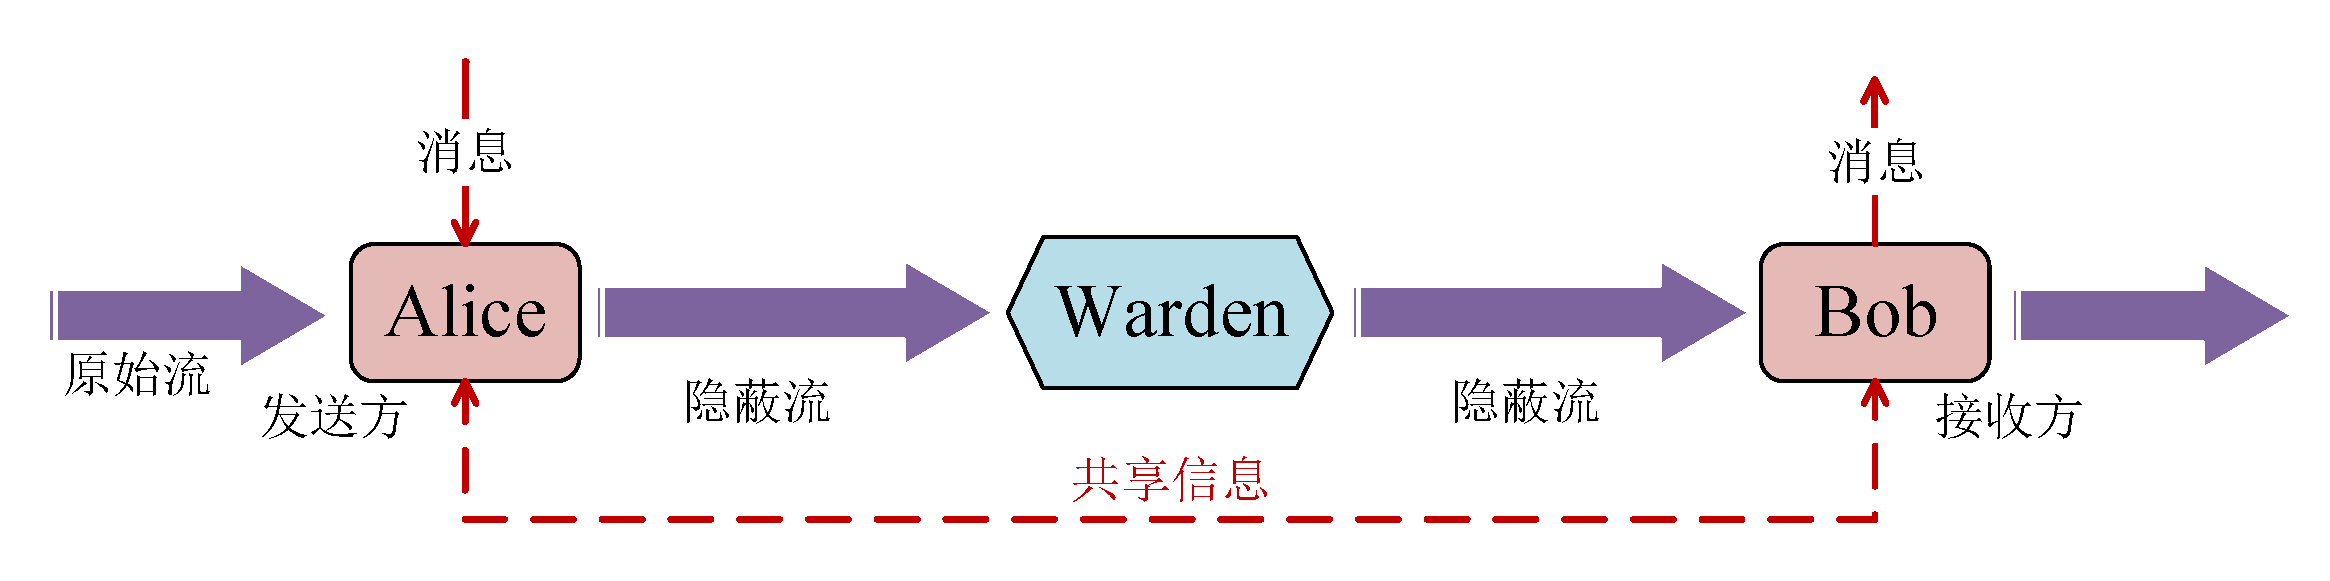
\includegraphics[width=\textwidth]{chapters/chapter1/figures/covert-channel.pdf}
        \caption{隐通道逻辑结构示意图}\label{fig:1:covert-channel}
	\end{figure}
}

对于隐通道的研究,主要集中在构建方法和检测方法两个方面。隐通道的逻辑结构示意如图\nref{fig:1:covert-channel},发送方和接收方利用共享信息,由发送方将宿主信道修改为隐蔽信道,接收方识别隐蔽信道中的特征信息,结合共享信息还原隐蔽消息。
隐通道最核心的环节,是如何实现调制过程,也就是将宿主信道修改为隐蔽信道的方式,这也是区分时间隐通道与存储隐通道的基本方法。
隐通道的检测方法,是针对特定类型的构建方法提出了,在应用范围上存在特定的局限性。
例如,基于IP(Internet Protocol)冗余字段的隐通道,修改了IP数据包头中的冗余字段,对宿主信道及上层应用不产生任何影响。对应的检测及消除措施,主要方式为扫描各字段的异常信息,并进行数据覆写。基于数据包顺序的隐通道,在构造过程中重新调整数据包序号,导致乱序现象出现,形成可检测的传输特征。通过数据包重排序,恢复正常顺序或再次打乱,在一定程度上破坏隐通道。\nupcite{ahsan2002practical}

%时间隐通道相对存储隐通道的优势是什么
在不同的应用场景中,隐通道有多种表现形式。在单主机环境下,隐通道的构建可以利用磁盘响应时间,通过影响磁盘访问队列\nupcite{130771},实现单主机中不同进程之间的隐蔽传输;时间隐通道JitterBug捕获键盘输入中的敏感信息,并通过松耦合的网络隐通道进行传输,在SSH(Secure Shell)、VNC(Virtual Network Computing)及RDP(Remote Desktop Protocol)等远程访问场景中具有可操作性\nupcite{shah2006keyboards}。
在以太网环境中,存储隐通道的构建多基于网络协议,类似于音频、视频中常用的隐写术,将消息块嵌入数据包中,如TCP(Transmission Control Protocol)包头中的冗余字段\nupcite{4317620}、IPv6包头中的AH及ESP字段\nupcite{10.1007/11767831_10};时间隐通道的构建,多基于数据包传输间隔及数据包发送顺序等。
相比于存储隐通道,时间隐通道在隐蔽性方面具有绝佳的优势,但受限于宿主信道的基础条件和网络噪声的影响,在信道容量及传输性能方面存在不足。因此,时间隐通道适用于少量核心消息的传输,存储隐通道适用于具有高性能传输需求的场景。

%移动互联网的兴起
随着第四代移动通信技术的广泛应用,以及移动智能终端的不断发展,移动互联网得到进一步发展,目前正由4G时代过渡到5G时代\nupcite{7470940}。
第四代移动通信技术,也就是LTE(Long Term Evolution)技术,在接入带宽、空口时延及负载能力等方面均得到了提升,使得面向移动互联网的应用得到繁荣发展。
不同于原有的移动通信技术,LTE网络在设计中采用了全IP网络模式\nupcite{6398495}。网络中的所有数据均封装为IP数据包,实现了更高的数据转发能力及更低的传输延迟;对不同应用、不同类型数据包的优化及优先级调度,提供了更好的用户体验;网络的鲁棒性得到提升,能够适应不同的应用场景。\nupcite{DBLP:journals/corr/abs-1810-02968}

%VoLTE是未来的趋势
由于LTE网络中取消了基于电路交换的通信技术,LTE网络中的语音通话必须向VoIP(Voice over IP)迁移,也就是VoLTE。通过基于数据包交换的传输方式,VoLTE在提供低延迟、高清晰度语音通话的同时,也支持低延迟的视频通话。
对于5G网络,音视频通话方案仍然会按照VoLTE的模式进行设计\nupcite{8412482},因此,对VoLTE的传输特征进行研究,并研究隐通道的构建环境,符合技术发展趋势。
得益于LTE核心网的传输保证,VoLTE通话质量优于第三方VoIP应用。通过提高VoLTE数据包优先级,即使是高负载的网络环境中,在通话延迟方面也具有显著优势;采用高效的编码方式,VoLTE在平衡通话质量的同时,有效降低了丢包率。\nupcite{anehill2012validating}

%研究VoLTE下时间隐通道构建方法,具有填补空白的意义
区别于VoIP应用,VoLTE由运营商保障端到端传输过程,形成了特有的传输环境,为时间隐通道提供了新的构建条件。受网络条件影响,VoLTE数据包类型、传输顺序及传输抖动均存在较强的规律性,一定程度上破坏了时间隐通道的构建基础。因此,在VoLTE环境中构建时间隐通道,需要改进构建方案,使得隐通道与宿主信道具有相同特征。研究基于主动丢包的时间隐通道方法,不仅扩充了隐通道构建方法,对于其它端到端传输环境也具有参考价值。